% Created 2025-09-15 Mon 00:02
% Intended LaTeX compiler: xelatex
\documentclass[14pt]{article}
\usepackage[a4paper, total={6.8132in, 9.6354in}]{geometry}
\usepackage{xcolor}
\usepackage{graphicx}
\usepackage{fvextra}
\usepackage{titlesec}
\usepackage{fontspec}
\usepackage{hyperref}
\usepackage{background}
\usepackage{shadowtext} % for drop shadow under cover titles

% Fonts
\setmainfont[Scale=1.2]{Fira Sans}
\setmonofont[Scale=1.0]{Fira Mono}

% Colors
\definecolor{gruv-bg}{HTML}{f9f5d7}
\definecolor{gruv-fg}{HTML}{3c3836}
\definecolor{gruv-accent}{HTML}{af3a03}
\definecolor{gruv-codebg}{HTML}{ffffff}
\definecolor{gruv-codetext}{HTML}{3c3836}
\definecolor{gruv-codeframe}{HTML}{ffffff}
\definecolor{covertext}{HTML}{3c3836}

\pagecolor{gruv-bg}
\color{gruv-fg}

% Hyperlinks
\hypersetup{
  colorlinks=true,
  linkcolor=gruv-accent,
  urlcolor=gruv-accent,
  citecolor=gruv-accent
}
\let\oldhref\href
\renewcommand{\href}[2]{\oldhref{#1}{\textbf{#2}}}

% Section formatting and spacing
\titleformat{\section}{\normalfont\LARGE\bfseries}{\thesection}{1em}{}
\setlength{\parskip}{0.7em}
\setlength{\parindent}{0pt}

% Code block appearance
\RecustomVerbatimEnvironment{Verbatim}{Verbatim}{
  fontsize=\large,
  breaklines=true,
  commandchars=\\\{\},
  bgcolor=gruv-codebg,
  formatcom=\color{gruv-codetext},
}
\usepackage{graphicx}
\usepackage{longtable}
\usepackage{wrapfig}
\usepackage{rotating}
\usepackage[normalem]{ulem}
\usepackage{capt-of}
\usepackage{hyperref}
\author{Kuzey Koç}
\date{\textit{<2025-09-10 Wed>}}
\title{Kubernetes}
\hypersetup{
 pdfauthor={Kuzey Koç},
 pdftitle={Kubernetes},
 pdfkeywords={},
 pdfsubject={},
 pdfcreator={Emacs 30.2 (Org mode 9.7.34)}, 
 pdflang={English}}
\begin{document}

\tableofcontents

% background setup for the cover page
\backgroundsetup{
  scale=0.8,
  angle=0,
  opacity=0.1,
  contents={
  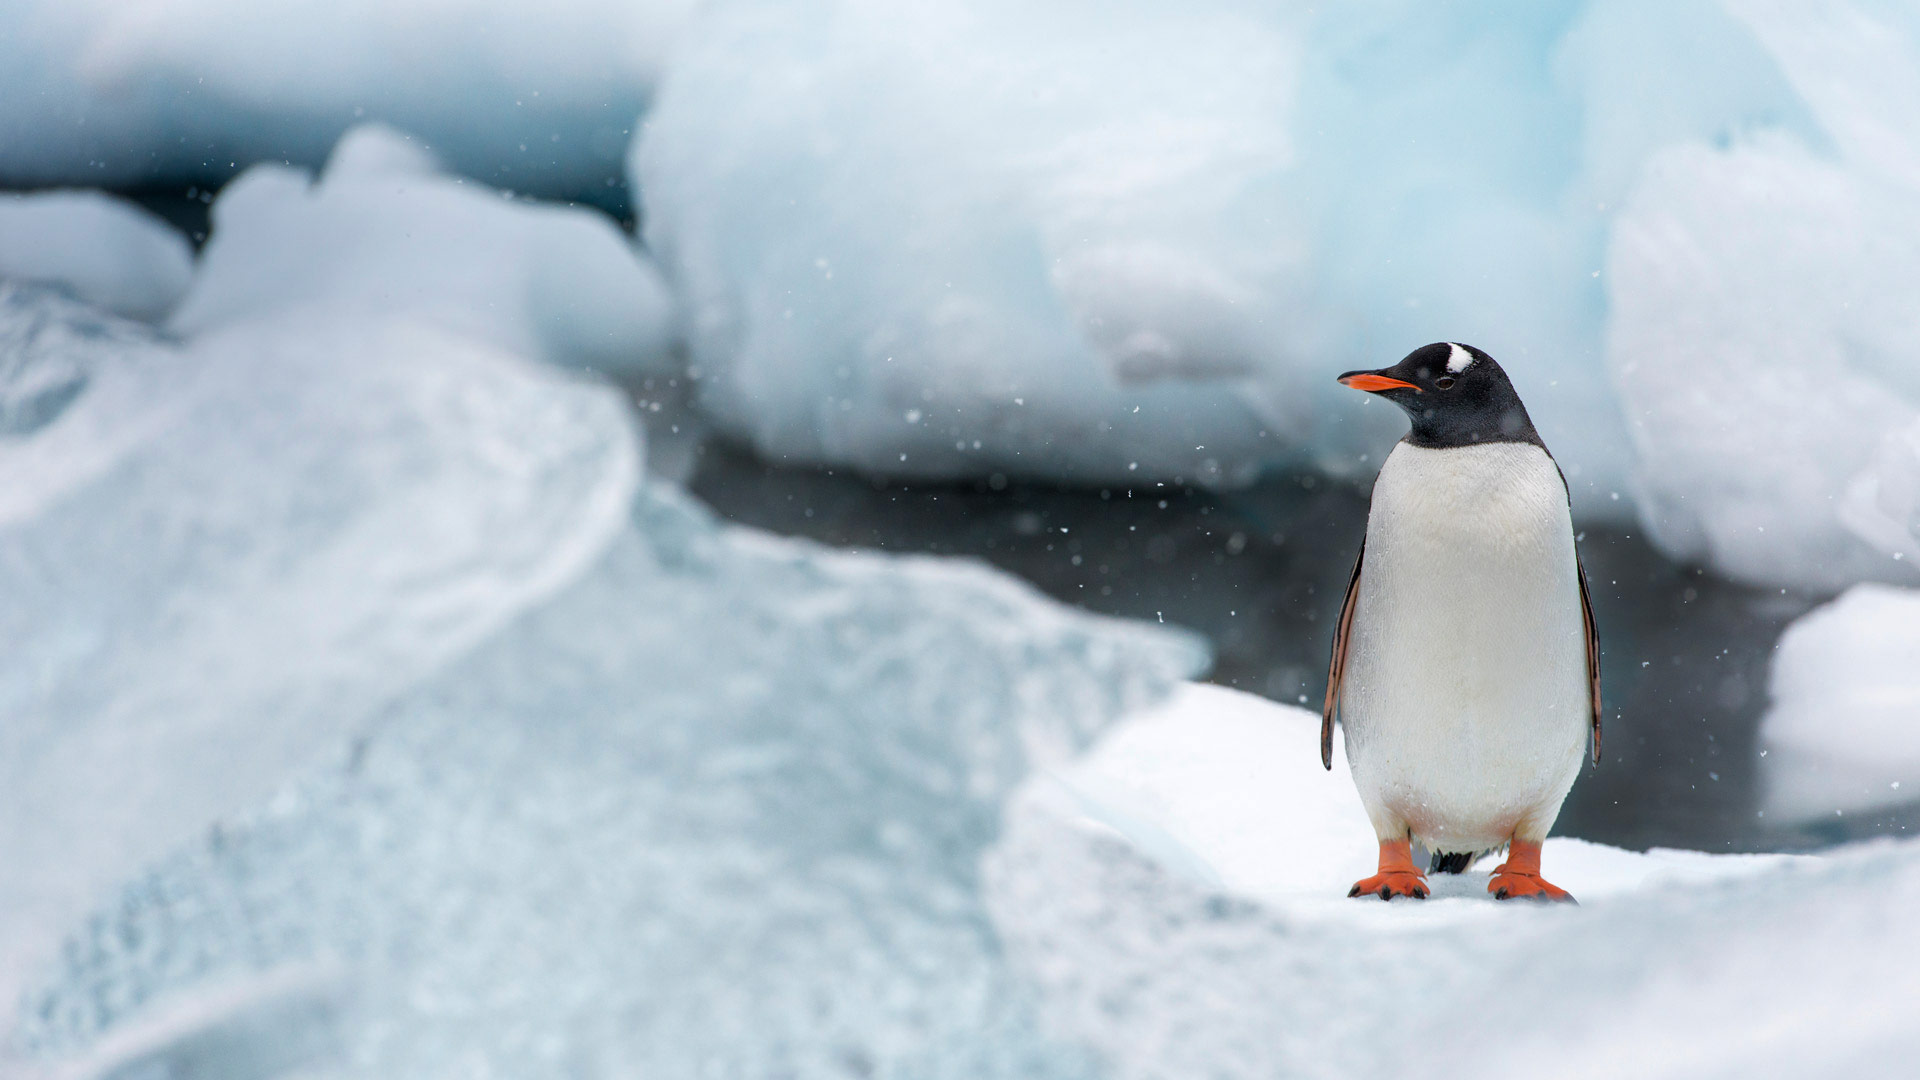
\includegraphics[
  width=1920,
  height=1080
  ]
  {/home/savolla/project/publishing/savolla.github.io/content/reference/kubernetes/featured.jpg}
  }
}

\definecolor{covertext}{HTML}{5d88de}

% cover page settings
\begin{titlepage}
  \BgThispage
  \color{covertext}
  \centering
  \vspace*{3cm}
  {\fontsize{25pt}{35pt}\bfseries DevOps Reference Series \par}
  \vspace{0.5cm}
  {\fontsize{60pt}{72pt}\bfseries Kubernetes \par}
  \vspace{1cm}
  {\fontsize{18pt}{20pt}\itshape by \par}
  \vspace{0.5cm}
  {\fontsize{23pt}{27pt}\itshape{\bfseries Kuzey Koç} \par}
  \vfill
\end{titlepage}

% set text color back to dark for main document
\color{gruv-fg}

% generate table of contents
\newpage
\tableofcontents
\newpage

You can get the PDF version of this article \href{file:///home/savolla/project/publishing/savolla.github.io/content/reference/kubernetes/index.pdf}{here} 📎
\section*{Applied Notes}
\label{sec:orge0c303e}
\section*{Notes}
\label{sec:org556b35b}
\begin{itemize}
\item kubernetesin mimarisinde 2 temel kavram vardır. \textbf{control plane} ve \textbf{worker node}
\begin{itemize}
\item control plane
\begin{itemize}
\item kubernetes spesifik proseslerin çalıştığı master.
\item control plane içinde çalışan önemli prosesler
\begin{itemize}
\item api server
\begin{itemize}
\item kısa ismi \textbf{api}
\end{itemize}
\item controller manager
\begin{itemize}
\item kısa ismi \textbf{c-m}
\item cluster içini sürekli izler ve bir sorun çıktığında onarır
\item bir pod ya da container öldü diyelim. hemen onu tamir eder. replicaset buna örnek verilebilir
\end{itemize}
\item scheduler
\begin{itemize}
\item kısa ismi \textbf{sched}
\item uygulamaları, worker nodelara dağıtır. bunu yaparken de workload ya da cpu ve ram kullanımlarına göre yapar
\end{itemize}
\item etcd
\begin{itemize}
\item key value store. yani kubernetes clusterının ayarlarını saklar. configürasyonu, her nodun statelerini vs tutar
\item ayrıca bir clusterın backupını almak istiyorsak etcd'den almamız gerekir
\end{itemize}
\end{itemize}
\item cluster içinde en az 2 control plane olması gerekir. çünkü biri düşerse diğer ayakta kalacak şekilde kurulması gerekir
\end{itemize}
\item worker node
\begin{itemize}
\item kullanıcı uygulamalarını çalıştığı ve control plane tarafından yönetilen serverlar
\end{itemize}
\end{itemize}
\item kubernetes için var olan web tabanlı arayüzler vardır. bunlardan biri \textbf{kubernetes dashboard}
\item kubernetes komponentleri
\begin{itemize}
\item pod
\begin{itemize}
\item kubernetesdeki en temel birimdir
\item bir ya da birden çok containerı barındırır
\end{itemize}
\item service
\begin{itemize}
\item pod içinde çalışan konteynerların kendi ip adresleri vardır ancak ephemeral oldukları için bu konteynerlar replicaset tarafından değiştirilir. bu olunca da ip adresi değişir. ip adresi değşse bile diğer uygulamaların bu pod içinde çalışan uygulamaya erişiminin devam edebilmesi için \textbf{service} diye bir k8s komponenti geliştirildi.
\item service, bir pod'a atanmış statik ip adresi gibi düşünülebilir
\item servis aynı zamanda bir \textbf{load balancer} gibi de davranır.
\end{itemize}
\item ingress
\begin{itemize}
\item pod içinde çalışan bir service browserdan erişmek istediğimizde ingres kullanabiliriz. burada ingress, service ile iletişim kurar. service ise gerekli konteynerın servisini ingresse açar.
\end{itemize}
\item configmap
\begin{itemize}
\item pod içinde çalışan uygulamanın ayarları ya da ortam değişkenlerini buraya yazabiliriz ve k8s buradan okuyup işlem yapabilir
\item configmap kullanmanın avantajı, bu değişkenleri dockerfile'a yazmayıp, uygulamayı her seferinde build etmememizi sağlar.
\end{itemize}
\item secret
\begin{itemize}
\item configmap gibi ancak daha hassas verileri saklamak için kullanılır. örneğin api tokenları, şifreler gibi.
\item secretlar \textbf{plain text} olarak etcd'de saklanır. api erişimi olan herkes bu bilgilere erişip secretları okuyup değiştirebilir. bu yüzden secretları encrypt etmek için 3rd party araçlar kullanılması gerekir. Vault gibi
\end{itemize}
\item volume
\begin{itemize}
\item pod içinde çalışan ve veri üreten konteynerların bu verileri \textbf{persistence} yapması için bir disk alanı gerekir. bunun için volumelar vardır. veritabanı gibi servislerin kesinlikle buna ihtiyacı vardır.
\item volume aynı makinede de saklanabilir, cloud providerların bir storage servisinde de saklanabilir
\end{itemize}
\item deployment
\begin{itemize}
\item pod, konteynerlar arası bir soyutlama yapıyorsa, deployment da podlar üstünden bir soyutlama yapan kubernetes konseptidir.
\item statei ya da bir volume'e ihtiyaç duymayan uygulamalar için kullanılır
\item genellikle direk podlar ile değil de deploymentlar ile çalışırız
\end{itemize}
\item stetefulset
\begin{itemize}
\item \textbf{sts} kısa ismi
\item database uygulamaları için özel olarak geliştirilmiştir. \textbf{mysql}, \textbf{mongodb}, \textbf{elasticsearch}. bu gibi uygulamalar \uline{her zaman stateful sets ile} deploy edilmelidir. deployment ile değil
\item database applikasyonlarını stateful set ile deploy etmek biraz uğraştırıcıdır. bu yüzden veritabanı gibi uyglamaları kubernetes clusterı dışında tutmak daha mantıklıdır. yani veritabanını yine deployment ile kurup asıl datbase bağlantısını dışardaki veritabanına göndermek en mantıklısıdır.
\end{itemize}
\end{itemize}
\item kubernetes has 3 different pluggable components
\begin{itemize}
\item CRI (container runtime interface)
\begin{itemize}
\item containerd and cri-o
\item docker was removed
\end{itemize}
\item CNI (container networking interface)
\begin{itemize}
\item k8s has k-proxy by default for cluster networking but there are different puggable services as well
\item flannel
\item calico
\item cilium
\end{itemize}
\item CSI (container storage intreface)
\begin{itemize}
\item this is for storage in cluster
\end{itemize}
\end{itemize}
\item \textbf{DaemonSet}
\begin{itemize}
\item \textbf{DaemonSet} her node'da çalışması gereken servislerin tanımlandığı bir deployment türüdür. Her bir node'da \uline{sistem düzeyinde} çalışması gereken servisler için kullanılır. Örnek olarak; \textbf{log toplama} (Fluentd, Logstash), \textbf{node monitoring} (prometheus node exporter), \textbf{container network interface} (calico, flanel) ve \textbf{security agents} gibi ``node'' ile ilgili olan servisler için kullanılır. \footnote{\href{https://chatgpt.com/}{ChatGPT}\label{org8a32457}}

\item Yeni bir node cluster’a eklenirse, DaemonSet otomatik olarak o node’da da bir Pod oluşturur. Node cluster’dan silinirse, ilgili Pod da silinir. İstersen sadece belirli label’lara sahip node’lara Pod yerleştirebilirsin (nodeSelector, affinity vb.). \textsuperscript{\ref{org8a32457}}

\item Bir daemonset oluşturmak için de şu örneğe bakabilirsin \href{daily/2025-09-10.org}{kubernetes daemonset file example}
\item \textbf{DaemonSet ve Deployment Farkları} \textsuperscript{\ref{org8a32457}}
\begin{center}
\begin{tabular}{lll}
özellik & DaemonSet & Deployment\\
\hline
pod sayısı & her node'a 1 tane & belirli sayıda (replicaset)\\
node'a bağlılık & evet & hayır\\
usecase & sistem/altyapı & aplikasyon\\
\end{tabular}
\end{center}
\end{itemize}
\item \textbf{Kubernetes Volumes}
\begin{itemize}
\item kubernetes does not give you data persistency out of the box \footnote{\href{https://www.youtube.com/watch?v=0swOh5C3OVM}{Kubernetes Volumes explained | Persistent Volume, Persistent Volume Claim \& S\ldots{}}}
\item \textbf{Persistent Volume}
\begin{itemize}
\item belongs to cluster itself. it is a dedicated disk
\end{itemize}
\item \textbf{Persistent Volume Claim}
\item \textbf{Storage Class}
\end{itemize}
\end{itemize}
\section*{Flashcards}
\label{sec:orgee62499}
\section*{Resources}
\label{sec:org148f22a}
\subsection*{Docs}
\label{sec:org6d7667b}
\begin{itemize}
\item \href{https://kubernetes.io/docs/home/}{Kubernetes Documentation | Kubernetes}
\end{itemize}
\subsection*{Videos}
\label{sec:orgb612b0a}
\begin{itemize}
\item \href{https://www.youtube.com/watch?v=2T86xAtR6Fo}{Complete Kubernetes Course - From BEGINNER to PRO - YouTube}
\item \href{https://www.youtube.com/watch?v=s\_o8dwzRlu4}{Kubernetes Crash Course for Absolute Beginners \{NEW\} - YouTube}
\end{itemize}
\subsection*{Books}
\label{sec:org1419352}
\subsection*{Articles}
\label{sec:orge6bb85d}
\end{document}
